% This file was created with tikzplotlib v0.10.1.
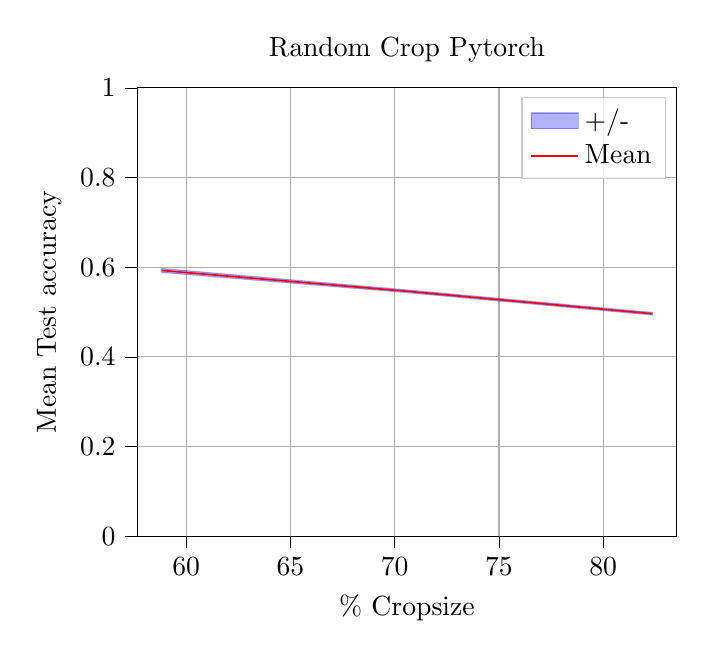
\begin{tikzpicture}

\definecolor{darkgray176}{RGB}{176,176,176}
\definecolor{lightgray204}{RGB}{204,204,204}

\begin{axis}[
legend cell align={left},
legend style={fill opacity=0.8, draw opacity=1, text opacity=1, draw=lightgray204},
tick align=outside,
tick pos=left,
title={Random Crop Pytorch},
x grid style={darkgray176},
xlabel={\% Cropsize},
xmajorgrids,
xmin=57.6470588235294, xmax=83.5294117647059,
xtick style={color=black},
y grid style={darkgray176},
ylabel={Mean Test accuracy},
ymajorgrids,
ymin=0, ymax=1,
ytick style={color=black}
]
\path [draw=blue, fill=blue, opacity=0.3]
(axis cs:58.8235294117647,0.59709293004768)
--(axis cs:58.8235294117647,0.588387069952319)
--(axis cs:70.5882352941177,0.543357834115176)
--(axis cs:82.3529411764706,0.493379375067802)
--(axis cs:82.3529411764706,0.499140624932198)
--(axis cs:82.3529411764706,0.499140624932198)
--(axis cs:70.5882352941177,0.549362165884824)
--(axis cs:58.8235294117647,0.59709293004768)
--cycle;
\addlegendimage{area legend, draw=blue, fill=blue, opacity=0.3}
\addlegendentry{+/-}

\addplot [semithick, red, opacity=1]
table {%
58.8235294117647 0.59274
70.5882352941177 0.54636
82.3529411764706 0.49626
};
\addlegendentry{Mean}
\end{axis}

\end{tikzpicture}
